\documentclass{template/socthesis}

\drafttrue
\jcmmfalse

\usepackage[T1]{fontenc} % evropské uvozovky
\usepackage{subcaption}
\usepackage{amsmath}
\usepackage{enumitem}
\usepackage{hyperref}
\usepackage{gensymb} % balíček symbolů
\usepackage{booktabs}
\usepackage{lmodern}
\usepackage{csquotes} % text lze uvést do uvozovek pomocí \enquote{text}, nepoužívat \enquote* !!!
\usepackage{textcomp}
\usepackage{pdfpages}

\usepackage[toc,page]{appendix}
\usepackage{color} % balíček pro obarvování textů
\usepackage{xcolor}  % zapne možnost používání barev, mj. pro \definecolor
\definecolor{mygreen}{RGB}{0,153,153} % nastavení barev odkazů 
\usepackage{listings} % balíček pro formátování zdrojových kódů 
\usepackage[author=,status=draft]{fixme} % vkládání poznámek  
% dva módy (status): draft (poznámky se zobrazují v PDF) / final (poznámky se nezobrazují v PDF)
\usepackage{graphicx}
\usepackage{multirow}
\usepackage{float}

\usepackage{expl3} % bibtex dependency, must be loaded prior to the bibtex
\usepackage[backend=bibtex,bibstyle=numeric,sorting=none,date=long,dateabbrev=false,texencoding=utf8,bibencoding=utf8,style=iso-numeric]{biblatex}

\usepackage[a4paper]{geometry}

\lstset { %
    language=C++,
    backgroundcolor=\color{black!5}, % set backgroundcolor
    basicstyle=\footnotesize,% basic font setting
}

\addbibresource{text.bib}
\nocite{*}

\titlecz{Sada materiálů pro podporu výuky strojírenské konstrukce v~SolidWorks}
\titleen{TITLEEN}
\author{Petr Štourač}
\field{12}
\school{Střední průmyslová škola a~Vyšší odborná škola Brno, Sokolská, příspěvková organizace}
\mentor{Ing. Václav Zavadil}
\mentorstatement{Ing. Václava Zavadila}

% Změňte, pokud se liší
%\region{Jihomoravský}
\placefooter{Brno 2021}

%\usepackage{hyperref} % balíček pro hypertextové odkazy
% \url{www.odkaz.cz}
% \href{http://www.odkaz.cz}{Text který bude jako odkaz}
% \hyperlink{label}{proklikávací_text} - odkaz na text 
% \hypertarget{label}{cíl_odkazu} - cíl odkazu 

\setlength{\parskip}{0.8em}
\begin{document}

\newgeometry{margin=2cm, top=4cm, bottom=2.5cm, left=2.5cm, includefoot}

\maketitle

\newgeometry{margin=2cm, top=2.5cm, bottom=2.5cm, left=2.5cm, right=2cm, includefoot}

\makecopyrightstatement{V~Brně}

\makethanks{\B{\textcolor{red}{PŠ: Poděkování sepísnu na závěr.}}}
% OLD: Děkuji svému školiteli Mgr. Miroslavu Burdovi za obětavou pomoc, podnětné připomínky a~hlavně nekonečnou trpělivost, kterou mi během práce poskytoval. Dále děkuji Kateřině Jelínkové za kontrolu gramatické správnosti a~korekce anglických textů. Kromě toho děkuji vyučujícím na naší škole za jejich podporu. Poděkování patří i Robotárně -- pobočce DDM Helceletova Brno za možnost využívání jejích prostor a~vybavení k~práci na SOČ.

\pagestyle{empty}

\section*{Anotace}
Počítačově asistovaný návrh je dnes nedílnou součástí strojírenské praxe.
Není proto divu, že se práce s~CAD programy běžně vyučuje na odborných školách s~technickým zaměřením.
Časová dotace těchto předmětů se zpravidla pohybuje okolo 2 až 4 hodin týdně, přičemž se liší jak mezi jednotlivými školami, tak i mezi obory.
Přesto, že se jedná o~jeden ze stěžejních předmětů, existuje pro něj velmi málo výukových materiálů.
Příprava výuky je tak čistě na samotných vyučujících.

Cílem této práce je usnadnit výuku konstrukce v~programu SolidWorks vytvořením edukativní sady zahrnující výukové videonávody, textové příručky a doplňkové materiály s~metodickými pokyny pro vyučující.

\subsection*{Klíčová slova}
SolidWorks, výuková sada, strojírenská konstrukce, výuková videa, podpora výuky

\vspace{20mm}

\section*{Annotation}
\B{\textcolor{red}{PŠ: Anotaci ještě přeložím, nicméně je to asi ta poslední věc na které teď záleží :-)}}

\subsection*{Keywords}
SolidWorks, educational kit, mechanical engineering, educational videos, teaching support

\newpage
\pagestyle{plain}

\setlength{\parskip}{0em}
\tableofcontents % vysází obsah

%%% Začátek práce
\setlength{\parskip}{0.8em}
\setcounter{figure}{0}
\setcounter{table}{0}
\newpage

% Uvod prace
\chapter*{Úvod}
\addcontentsline{toc}{chapter}{Úvod}
Počítačově asistovaný návrh je dnes nedílnou součástí strojírenské praxe.
Není proto divu, že se práce s~CAD\footnote{Computer aided design - počítačově asistovaný design} programy běžně vyučuje na odborných školách s~technickým zaměřením.
Časová dotace těchto předmětů se zpravidla pohybuje okolo 2 až 4 hodin týdně, a liší se mezi jednotlivými školami, i mezi obory.
Přestože se jedná o~jeden ze stěžejních předmětů, existuje pro něj velmi málo výukových materiálů.
Příprava materiálů proto velmi záleží přímo na samotných vyučujících.

Pro výuku SolidWorks\cite{SOLIDWORKS}, který je jedním z~nejčastěji používaných CADů aktuálně existuje pouze jedna učebnice.
Na druhou stranu videonávodů existuje mnohem více, zpravidla však nejsou primárně určeny pro použití ve výuce.

3D modelování mne odjakživa bavilo, při nástupu na střední školu pro mne tedy nešlo o~nic nového.
Totéž se ovšem nedalo říci o~spoustě mých spolužáků, kteří s~ním měli velké problémy.
Často jsem se proto dostával do situace, kdy se blížil termín odevzdání nějakého projektu a já jsem byl doslova \enquote{zasypáván} dotazy spolužáků na to, jak vymodelovat nějaký prvek, popřípadě součást.
Pokaždé, když se nějaký konkrétní dotaz opakoval, jsem přemýšlel, zda by neexistoval efektivnější způsob, jak spolužákům pomoci.
Začal jsem proto odpovědi společně s~ukázkami v~SolidWorks natáčet.
V~této počáteční fázi jsem však netušil, jak se celý projekt s přibývajícím časem rozroste.

Postupně jsem začal uvažovat nad tím, zda by tato videa bylo možné využít i při výuce.
Konzultoval jsem tento nápad s~Ing. Zavadilem, který na naší škole učí předmět konstrukční cvičení.
Shodli jsme se, že vytvoření výukových videí by ulehčilo práci nejen studentům, ale i vyučujícím.

V~průběhu tvorby těchto videí jsem projekt postupně rozšiřoval a přidával další, neméně důležité prvky.
Prvním z~nich byly tisknutelné textové materiály.
Uvědomil jsem si totiž, že ne každému studentovi může audiovizuální forma předávání informací vyhovovat.
K~výukovým videím jsem z toho důvodu vytvořil doplňkové vytisknutelné materiály, které předávají obsah videí v~textové podobě.
Textové materiály jsem postupně rozšířil i o~otázky a úkoly, pomocí kterých si může student dané téma zopakovat, nebo je může vyučující použít pro ověření znalostí studenta.
Vznikla tak komplexní sada materiálů pro podporu výuky strojírenské konstrukce v~SolidWorks.
Proto, aby byla celá sada snadno a rychle dostupná jsem následně přidal i webový portál P3D, na kterém jsou všechny její dílčí části volně k~dispozici.

Důležité je zmínit, že pro tvorbu určité součásti, nebo prvku\footnote{Každý díl, popřípadě součást se skládá z určitých prvků, které definují její tvar} může existovat více než jedno konkrétní řešení a není jasně dáno, které z~nich je správné.
Rozdíl mezi řešeními spočívá především v jejich časové náročnosti a efektivitě.
Celá výuková sada má tedy za cíl ukázat studentům optimální způsob řešení daného problému, a následně jeho pochopení ověřit pomocí doplňujících úkolů a otázek.
V~případě, že student kvůli přibývajícímu počtu postupů některý z~nich zapomene, může se snadno vrátit a zpětně shlédnout video, které problematiku popisuje, nebo nahlédnout do souvisejících doplňkových materiálů.

\newpage
 %%% Asi HOTOVO, možná ještě něco doplním...

\chapter{Cíle práce}

\begin{enumerate}[topsep=0pt]
    \setlength\itemsep{0em}
    \item \B{Usnadnění výuky strojírenské konstrukce v~programu SolidWorks}
    
    \item \B{Hlavní cíle:}
    \begin{enumerate}[topsep=0pt]
        \setlength\itemsep{0em}
        \item Vytvoření sady videonávodů na práci s~různými prvky v~konstrukčním programu SolidWorks
        \item Sestavení doplňkových materiálů v~tištěné podobě, které jsou využitelné zejména v~prezenční výuce a jsou obohacené o~doplňující otázky a úkoly
        \item Připravení metodických pokynů pro vyučující k~práci s~těmito materiály
        \item Vytvoření platformy (webového portálu), na kterém budou tyto materiály volně k~dispozici pro studenty i učitele
        \item Spolupráce s~vyučujícími strojírenských předmětů na implementaci vytvořených materiálů do výuky
    \end{enumerate}

    \item \B{Sekundární cíle:}
    \begin{enumerate}[topsep=0pt]
        \setlength\itemsep{0em}
        \item Zjišťování využitelnosti výsledků práce mezi studenty 
        \item Spolupráce se studenty a vyučujícími na obsahu vytvořených materiálů (volba témat, kontrola správnosti apod.) 
    \end{enumerate}
\end{enumerate}
 %%% HOTOVO

\chapter{Dosavadní výuka strojírenské konstrukce}
\noindent \B{OSNOVA:}
\begin{itemize}[topsep=0pt]
    \setlength\itemsep{0.05em}
    \item jak výuka probíhá
    \item co mají studenti aktuálně k dispozici
\end{itemize} %%% Kratší kapitola, dopíšu do 25. bř

\chapter{Názorně - demonstrační pomůcky}
V~této kapitole se zaměřuji na trendy ve výuce technických předmětů a metody při ní využívané.

\section{Trendy ve výuce technických předmětů}
Výuka technických předmětů vyžaduje velmi specifický přístup.
Aby student látku správně pochopil, je kromě teoretických znalostí nezbytná i ukázka jejich aplikace.
Nejběžnějším způsobem této ukázky jsou modely dílů, nebo mechanismů speciálně upravených tak, aby si student vytvořil komplexní představu o~jejich funkci a účelu.
Tyto ukázkové modely však mají své nevýhody. 
Jedna z největších nevýhod bývá patrná převážně při předvádění větších mechanismů.
Často totiž ve výuce není prostor ani čas na detailní rozebrání modelu, a studenti tak často vidí jen zevnějšek, nebo některé vnitřní části skrze speciálně prořezané otvory.
Tím může být vytvoření komplexnější představy pro studenta značně ztíženo.

Stále častěji se proto využívá počítačových vizualizací, nebo animací, které umožňují celý model pomocí několika kliknutí snadno rozebrat, nebo některé části skrýt. 
Díky tomu mohou studenti vidět funkci některých mechanismů i zevnitř, což je ve srovnání s modely nespornou výhodou.

Běžná bývá také praktická výuka vyučovaná v~dílnách, popřípadě laboratořích, kde dochází k~propojení teorie s~praxí, jako například u technologie třískového obrábění.
Studenti se nejdříve v~hodinách strojírenské technologie dozví, jak třískové obrábění probíhá, jeho princip a metody.
Následně si studenti mohou v~dílnách toto obrábění sami prakticky vyzkoušet na soustruhu, nebo na frézce.

\section{Předvádění a pozorování}
V~souvislosti s~již zmíněnými ukázkovými modely se často aplikuje právě metoda předvádění a pozorování.
Jedná-li se o~fyzický model, studenti si jej mohou prohlížet, přičemž vyučující o~daném modelu provede výklad.
U~elektronických modelů nebo animací je situace podobná.
Rozdíl je v tom, že model není fyzicky přítomen v učebně, ale animace, popřípadě vizualizace je promítána na plátno.

Tato metoda je vhodná zejména pro výuku technických předmětů, kde potřebují studenti znát princip, funkci a účel určité součásti, nebo mechanismu. 
Pro výuku konstrukce v~CAD programech je vhodná jen okrajově -- studenti potřebují vědět, jak mechanismus funguje, aby s~ním v~SolidWorks mohli poté správně individuálně pracovat.
Obvykle se však jedná pouze o vizuální ukázku funkce, samotný postup tvorby tohoto mechanismu studentům popíše až instruktáž.

\section{Instruktáž}
Ve školním prostředí je instruktáž jednou z~často používaných názorně - demonstračních výukových metod.
Pomocí vizuálních, zvukových, popřípadě audiovizuálních podnětů umožňuje studentům si osvojit nové znalosti a v~kombinaci s~metodami praktickými je uplatnit v praxi.
Skládá se zpravidla z~ukázky doplněné komentářem -- takzvanými instrukcemi.

\noindent V~závislosti na používaných podnětech je možné rozlišit několik typů instruktáže:
\begin{itemize}[topsep=0pt]
    \setlength\itemsep{0em}
    \item \B{Slovní instruktáž} využívá verbálních instrukcí k~popsání vysvětlované činnosti.
    \item \B{Audiovizuální instruktáž} kombinuje slovní instruktáž s~praktickou ukázkou, nebo vizuálními podklady (obrázky, video).
    \item \B{Písemná instruktáž} je spojením slovní instruktáže a psané formy doplněné o~ilustrace.
\end{itemize}

Instruktáž je nejčastěji využívána právě při výuce konstrukce v~SolidWorks, při které vyučující nejprve nějaký postup předvede a popíše, a poté si jej studenti sami vyzkoušejí.

\subsection{Instruktáž v~jednotlivých částech výukové sady}
Jak výuková videa, tak i vytisknutelné materiály tvoří určitou formu instruktáže.
V~případě výukových videí se jedná o~instruktáž audiovizuální, spojující mluvený komentář (slovní instrukce) s~názornou ukázkou.
Tyto dvě části se navzájem doplňují.
Zatímco názorná ukázka daný postup předvádí, mluvený komentář přidává doplňující informace a usměrňuje pozornost studenta.

Tisknutelné materiály jsou poté formou písemné instruktáže.
V~textové podobě jsou zde přítomny slovní pokyny doplněné o~ilustrace částí postupu, které jsou pro tento typ úloh stěžejní.

\newpage %%% Dopíšu do 2. dubna - bude potřeba intenzivní kopání

\chapter{Dílčí části výukové sady}
\large \B{Note: \textcolor{mygreen}{Název sekce se ještě nejspíš změní. Popíšu zde jednotlivé části projektu, jejich formát, co obsahují a možnosti využití.}}

\section{Výukové videonávody}

\section{Textové návody}

\section{Webový portál P3D}

\section{Doplňující materiál s otázkami a úkoly} %%% Napíšu do 24. bř, možná ještě něco doplním později

\chapter{Integrace do výuky a využití}
Již v~průběhu psaní této práce jsou materiály z~výukové sady využívány vyučujícími a studenty naší školy.
Kromě nich je využívají i někteří vysokoškoláci.

\section{Sledovanost v~číslech}
Ke dni 7. 4. 2021 se celkový počet zhlédnutí všech veřejných videí pohybuje okolo dvou tisíc (přibližný počet je 1875).
Obecně nejsledovanějším videem je návod na instalaci SolidWorks SDK 2020/2021 se 720 zhlédnutími, které bylo distribuováno primárně mezi studenty naší školy.
Za ním se nachází video zaměřené na modelování ozubeného kola s~přímým ozubením s~352 zhlédnutími.

Návštěvnost webového portálu P3D se aktuálně pohybuje v~řádu stovek.
Ke dni 7. 4. 2021 zaznamenal tento web přibližně 500 návštěvníků.

\section{Distanční výuka}
Výuková videa našla při distanční výuce podstatné využití.
Videokonferenční programy nezaručují dostatečně vysokou kvalitu přenosu obrazu ani zvuku, kvůli čemuž by musel vyučující ukázku postupu při výpadku na straně studentů často opakovat.
Učitelé na naší škole proto v~některých případech vlastní ukázky zcela nahrazují odkazováním na mnou vytvořená výuková videa a materiály, jelikož jsou schopny tyto ukázky plně zastoupit.
Sami studenti tyto materiály využívají při práci na svých projektech, jelikož kvůli absenci prezenční výuky nemají možnost pracovat v~hodinách za přítomnosti učitele a nemohou se na něj tedy obrátit s~žádostí o~pomoc.
Ti zvídavější z~nich se pomocí mých materiálů mohou učit nové postupy, ke kterým v~běžné výuce ještě nedošli.

\section{Využití materiálů v~prezenční výuce}
K~praktickému využití v~prezenční výuce bohužel z~důvodu celosvětové pandemie zatím nedošlo. 
I~přesto je jejich implementace do výuky strojírenské konstrukce plánovaná přinejmenším na naší škole.
Většina vyučujících je začne s~obnovením prezenční výuky využívat a v~příštím roce bych rád praktickou aplikaci svých materiálů dále rozšířil.

Vzhledem k~tomu, že jsou všechny materiály volně dostupné, jejich využití je proto možné i na jiných školách.
S~tím se pojí i velmi snadné začlenění do výuky.
Vyučující nemusí nic složitě hledat -- na webových stránkách snadno a rychle najde vytisknutelné materiály i výuková videa.
Textové materiály samozřejmě není nutné používat jen v~papírové podobě. Studentům je může snadno rozeslat ve formátu PDF, popřípadě může jen odkázat na webové stránky \href{https://www.p3dportal.cz}{www.p3dportal.cz}.

Způsobů využití mojí výukové sady v~prezenční výuce existuje celá řada.
Vyučující upřednostňující textovou formu mohou studentům vytisknout a rozdat materiály nebo jim je snadno rozeslat.
Pokud je v~učebně k~dispozici projektor, mohou promítat výuková videa, případně nechat studenty, aby je sledovali samostatně na svých počítačích.
Další možností je kombinované využití výukových videí a tištěných materiálů, kdy vyučující pomocí projektoru nechá studenty zhlédnout video, následně jim rozdá vytisknuté materiály a nechá je vypracovat úkoly a otázky, které jsou v~nich obsaženy.
 %%% Dopíšu do 2. dubna

% Zaver prace
\chapter*{Závěr}
\addcontentsline{toc}{chapter}{Závěr}
V~průběhu práce jsem vytvořil komplexní výukovou sadu, kterou je možné snadno používat přímo ve výuce strojírenské konstrukce v~SolidWorks na středních průmyslových školách.
Celá tato výuková sada se skládá jednak z~výukových videí sloužících jako audiovizuální instruktáž práce s~různými prvky a funkcemi v~programu SolidWorks.
Druhou, neméně důležitou částí jsou tisknutelné materiály, využitelné zejména při prezenční výuce, které obsahují doplňující otázky a úkoly.
Díky nim si může student dané téma zopakovat a vyučujícímu umožňuje ověřit znalosti tohoto studenta. 

Ke dni odevzdání této práce vzniklo již 11 výukových videí a pro každé z~nich existuje i textová verze obsažená v~tisknutelných doplňkových materiálech.
Tyto materiály jsou doplněny o~otázky a úkoly, sloužící k~procvičení daného tématu, případně ověření znalostí studenta.
Ve variantě těchto textových materiálů pro vyučující jsou navíc přidány doporučení k~aplikaci ve výuce, upozornění na problematické části postupu a řešení otázek a úkolů.

Již nyní jsou mé materiály volně dostupné na webovém portálu P3D (\href{https://www.p3dportal.cz}{www.p3dportal.cz}) a jsou při nynější distanční výuce využívána nejen studenty a vyučujícími na naší škole, ale i některými vysokoškoláky.
Aplikace materiálů do prezenční výuky je na naší škole plánována s~návratem studentů do škol.

Témat, která by si zasloužila začlenění do mé výukové sady, existuje obrovské množství.
Vzhledem k~tomu, že mne tato tvorba opravdu baví a zároveň má užitek pro studenty i vyučující, plánuji v~ní pokračovat i nadále.
Během následujících měsíců plánuji sadu rozšířit o~materiály zabývající se například tvorbou plechových dílů, svařovaných konstrukcí, prvků technické dokumentace a mnoha dalších.

Věřím, že mnou vytvořená výuková sada se bude dále rozrůstat a bude skvělým pomocníkem studentů i vyučujících.
\newpage %%% Jako vždy píšu až na konec...
\newpage

\appendix
\addcontentsline{toc}{chapter}{Přílohy}

% Prilohy
\chapter{Seznam již vydaných videí} \label{released-videos}
Tato příloha obsahuje kompletní seznam videí vzniklých v~rámci projektu P3D vč. odkazů rozdělených dle jednotlivých témat. \newline
\noindent\It{Pozn.: při kliknutí na odkaz budete přesměrování na stránku korespondujícího videa}.

\section{Instalace a zprovoznění SolidWorks SDK} \label{videa-instalace}
\href{https://go.p3dportal.cz/inst-sdk2021}{Instalace a první spuštění SolidWorks SDK 2020/2021 (go.p3dportal.cz/inst-sdk2021)} \newline
\href{https://go.p3dportal.cz/sablony-vid}{Instalace šablon a knihoven norm. dílů ze Sokolské (go.p3dportal.cz/sablony-vid)} \newline
\href{https://go.p3dportal.cz/GkkCtx}{Aktivace Realview na necertifikované grafické kartě (go.p3dportal.cz/realview)} \newline

\section{Základy modelování} \label{videa-modelovani}
\href{https://go.p3dportal.cz/pruzina}{Jednoduchá pružina (go.p3dportal.cz/pruzina)} \newline
\href{https://go.p3dportal.cz/oz-kolo}{Ozubené kolo s~přímým čelním ozubením (go.p3dportal.cz/oz-kolo)} \newline
\href{https://go.p3dportal.cz/vykresove-ozk}{Ozubené kolo pro výkres - obálka (go.p3dportal.cz/vykresove-ozk)} \newline
\href{https://go.p3dportal.cz/jr-rk}{Jednořadé řetězové kolo (go.p3dportal.cz/jr-rk)} \newline
\href{https://go.p3dportal.cz/perodr-na}{Drážka pro pero v~náboji (go.p3dportal.cz/perodr-na)} \newline
\href{https://go.p3dportal.cz/perodr-hr}{Drážka pro pero na hřídeli (go.p3dportal.cz/perodr-hr)} \newline

\newpage

\section{Výkresová dokumentace} \label{videa-vykresy}
\href{https://go.p3dportal.cz/popisove-pole}{Popisové pole a už. vlastnosti na výkrese (go.p3dportal.cz/popisove-pole)} \newline
\href{https://go.p3dportal.cz/dwg-perodr-na}{Výkres drážky pro pero v~náboji (go.p3dportal.cz/dwg-perodr-na)} \newline
\href{https://go.p3dportal.cz/dwg-perodr-hr}{Výkres drážky pro pero na hřídeli (go.p3dportal.cz/dwg-perodr-hr)} \newline

\section{Práce se sestavami} \label{videa-sestavy}
\href{https://go.p3dportal.cz/prejm-dilu}{Přejmenování dílu v~sestavě (go.p3dportal.cz/prejm-dilu)} \newline
\href{https://go.p3dportal.cz/pack-and-go}{Přesun sestavy pomocí Pack and Go... (go.p3dportal.cz/pack-and-go)} \newline

\chapter{Tisknutelné materiály}
Součástí příloh této práce jsou i doplňkové materiály ve ve variantě pro studenty, ke kterým je na závěr doplněn krátký úsek z materiálů pro vyučující.
Vzhledem k tomu, že s přibývajícím množstvím výukových videí se rozrůstají i textové materiály, je jejich pravidelně aktualizovaná verze k dispozici na \href{https://go.p3dportal.cz/textmat-st}{go.p3dportal.cz/textmat-st}.
Verze přiložená v této práci je aktuální k datu 8. 4. 2021.
Pro přehlednost jsou tyto materiály umístěny až za formální konec práce, kterým je seznam obrázků na straně \pageref{listoffigures}.



\setlength{\parskip}{0em}
\printbibliography[title=Literatura]
\addcontentsline{toc}{chapter}{Literatura}

\listoffigures \label{listoffigures}
\addcontentsline{toc}{section}{Seznam obrázků}

%\listoftables
%\addcontentsline{toc}{section}{Seznam tabulek}

\setlength{\hoffset}{0mm}
%%% ODKOMENTOVAT PŘED FINÁLNÍ KOMPILACÍ!!!
\addcontentsline{toc}{chapter}{Příloha: Tisknutelné materiály pro studenty}
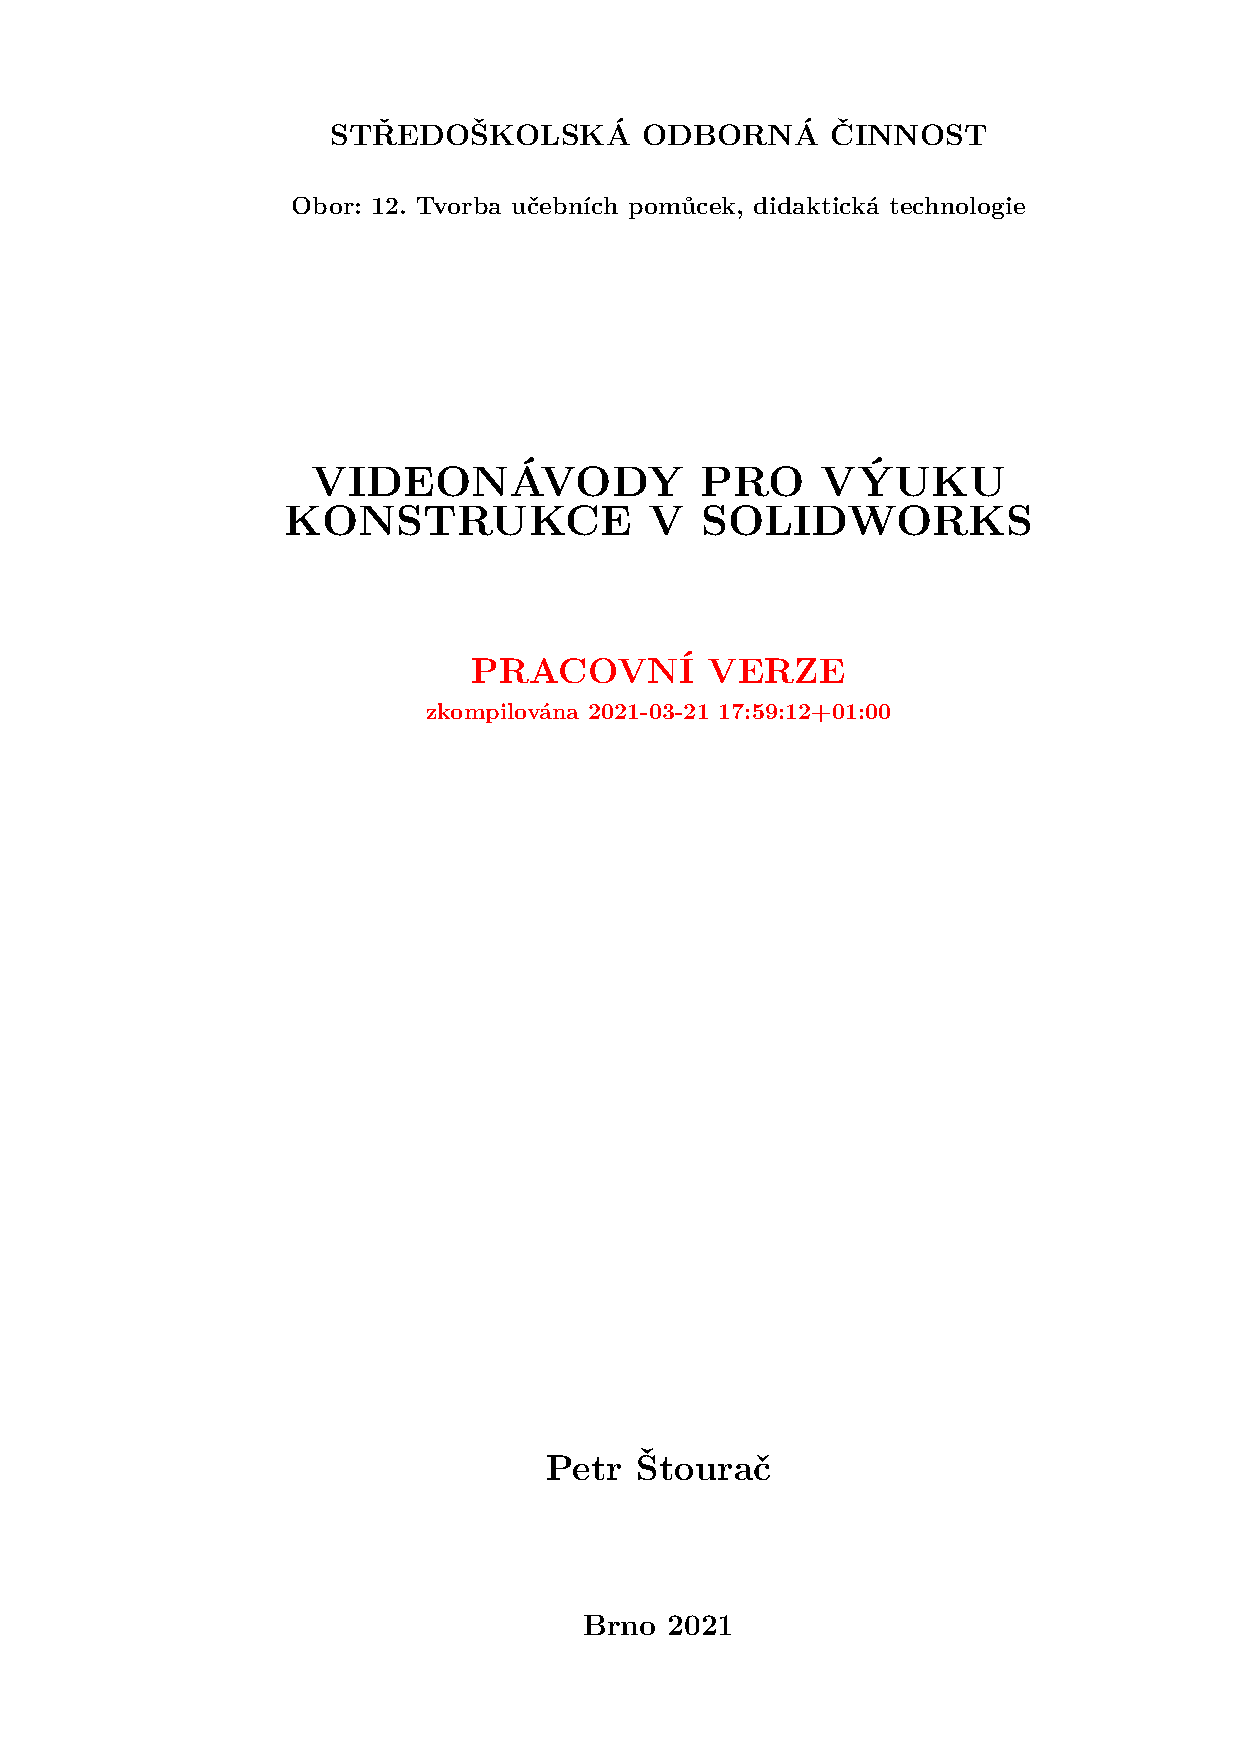
\includepdf[pages=-]{P3D-auxmaterials/text.pdf}

Zde budou ještě materiály pro učitele...
\addcontentsline{toc}{chapter}{Příloha: Tisknutelné materiály pro vyučující}

\end{document}
